\begin{figure*}[!htbp]
  \centering  
  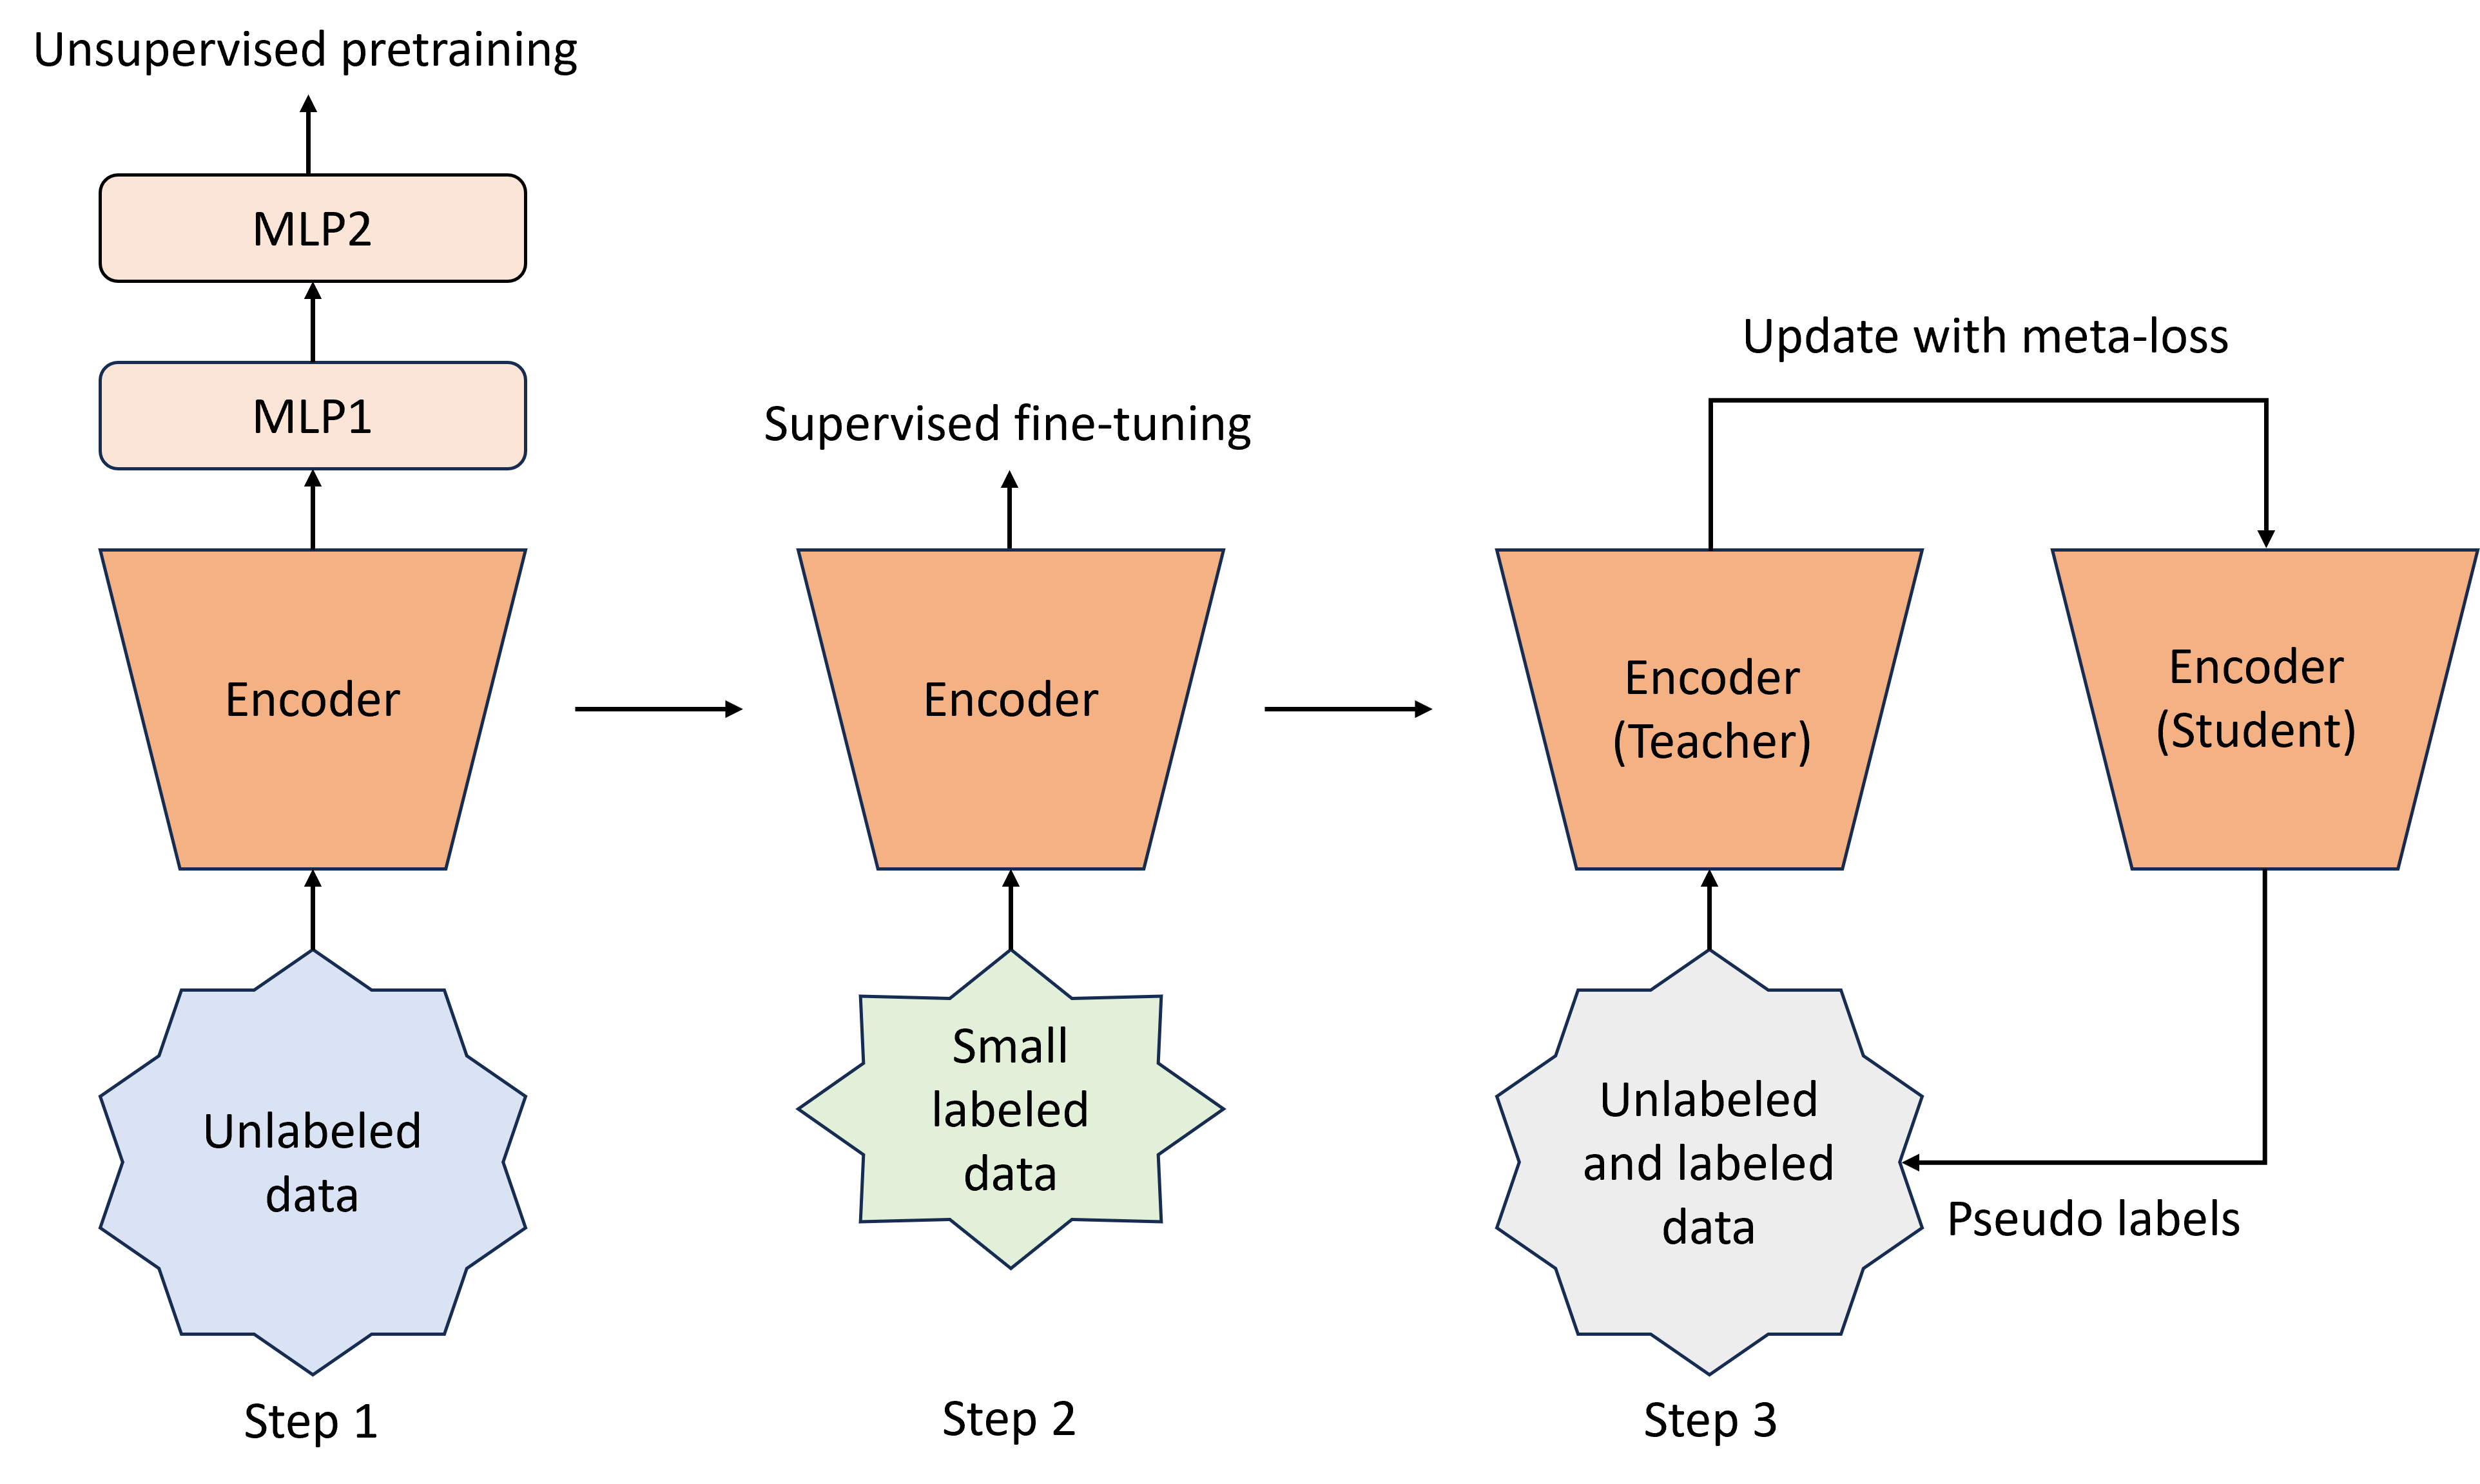
\includegraphics[width=0.75\textwidth]{images/flow.png}
  \caption{\textbf{RLPL flowchart.} 
  RLPL has two levels of unlabeled data utilization. First, it employs unsupervised representation learning. Second, We obtain a highly accurate fine-tuned classifier using only a handful of label data. Lastly, through pseudo labelling using teacher-student networks, both initialized from superior supervised backbone, we improve the classifier further.}
  
% (\textcolor{red}{In this figure, should we indicate the Teacher network with $f_{\theta_T}$, and the Student network with $f_{\theta_S}$? We can mention here at the beginning, $\theta=\theta_T=\theta_S$})
  
  \label{fig:flow}
\end{figure*}
\section{Introduction}

While supervised machine learning algorithms thrive on labeled data, manually annotating this data can be both time-consuming and costly. In contrast, unlabeled data is often readily available and abundant. Although it lacks explicit labels,  unlabeled data still holds valuable information that machine learning models can harness. Semi-supervised learning bridges this gap by extracting meaningful patterns from unlabeled data, compensating for the limited labeled datasets \cite{kingma2014semi}. It achieves this by utilizing the unlabeled data to uncover latent representations—underlying structures and relationships that aren't directly observable. Semi-supervised learning can enhance model performance by incorporating these latent representations, even when labeled data is scarce \cite{devillers2024semi, kutuzova2021multimodal}.

Contrastive learning \cite{chuang2020debiased, fan2023contrastive} has been proven effective in learning the data representation using the unlabeled sample. However, they require negative samples to avoid representational collapse \cite{aghajanyan2020better} and hence were plagued by the problem of mining negative samples \cite{radenovic2023filtering}. There are no apparent methods to obtain effective negative samples, and the presence of higher negative samples than positive ones creates an imbalance \cite{kalantidis2020hard}. Subsequently, contrastive learning methods rely on a large batch size \cite{yang2023batchsampler} to achieve good performance, leading to expensive computational needs.

Representation Learning (RL) methods, such as Bootstrap Your Own Latent (BYOL), SimSiam, and Barlow Twins solve the problem of negative samples by learning representation from the positive class alone. While these methods achieve impressive results with large batch sizes (typically 1024-4096), their performance degrades significantly with smaller batches. This degradation occurs because larger batches provide better gradient estimates and more diverse learning signals, which are crucial for stable representation learning. However, the high memory requirements of large batches make these methods impractical for resource-constrained environments.

Our analysis reveals that the performance drop in existing methods with smaller batches (8-128) stems from two key factors: (1) unstable gradient estimates leading to suboptimal convergence, and (2) limited diversity in the learning signals within each batch. RLPL addresses these challenges through a novel approach that maximizes information utilization from each sample, enabling stable learning even with smaller batches. Through extensive experimentation across different batch sizes, we demonstrate that RLPL maintains consistent performance, showing only a marginal accuracy drop with reduced batch sizes.

Unlabeled data, typically unused in downstream tasks, can enhance performance when leveraged through a model with strong initialization. Pseudo-Labels (PL) \cite{lee2013pseudo} employ a confidence threshold to selectively include those unlabeled samples for which the classifier demonstrates high certainty in its predictions. RL offers an effective initialization, enabling improved model performance and confident pseudo-labeling. However, a notable challenge arises when incorrect pseudo labels are assigned, leading to a degradation in classifier accuracy due to learning from corrupted data. RLPL addresses this issue by refining the pseudo labels through a teacher-student network. This process enhances the teacher network, making it a better model to guide the student network, thereby generating more accurate pseudo labels and boosting overall performance.



% Meta Pseudo Labels (MPL) \cite{Pham_2021_CVPR} addresses pseudo-labeling challenges by iteratively refining PLs through teacher-student \cite{hinton2015distilling} networks, where the teacher network updates itself based on feedback from the student network. Our advanced pseudo-labeling approach focuses on strengthening the teacher network, making it a better model to guide the student network. This improvement helps generate more accurate PLs, which boosts overall performance.

Typical RL methods demand extensive computational resources, such as hundreds of TPUs over several days. Additionally, pseudo-labeling is another memory-heavy method as it uses two networks simultaneously. These requirements are challenging in scenarios where fast, efficient models are needed, like in autonomous vehicles or edge computing \cite{guo2023architecture}. To address these limitations, we implement RLPL on a more manageable batch size and a shallower network, leveraging just two Nvidia 4090 GPUs. Our study shows that RLPL, even without the usage of pseudo labeling, achieves higher accuracy with a batch size of 64, outperforming BYOL with a 128 batch size. Remarkably, RLPL consistently outperforms other RLs with a ResNet18 classifier. RLPL yields average accuracy improvements of \textbf{2.7\%}, \textbf{9.22\%}, and \textbf{4.16\%} that the closest contemporary method on the STL-10, CIFAR-10, and SVHN datasets, respectively.

% Our study shows that RLPL achieves competitive accuracy even with a batch size of 64, matching or outperforming other methods using much larger batches. While methods like FixMatch and MixMatch report higher accuracies (94.83% and 94.41% respectively on STL-10) with large batches (4096), they show significant degradation with smaller batches. In contrast, RLPL maintains robust performance across batch sizes, making it particularly suitable for resource-constrained scenarios. With ResNet18 as the backbone, RLPL yields average accuracy improvements of \textbf{2.7\%}, \textbf{9.22\%}, and \textbf{4.16\%} over the closest contemporary method on the STL-10, CIFAR-10, and SVHN datasets, respectively, when using comparable batch sizes.

Figure \ref{fig:flow} illustrates our framework. In summary, our work contains the following contributions:

\begin{itemize}

\item Our approach cleverly leverages most information from the inputs, leading to enhanced global representation learning. By making this strategic adjustment, our model achieves improved representations with a smaller batch size, ultimately achieving higher accuracy in the downstream tasks.

\item During the downstream task, we utilize unlabeled samples a second time with pseudo labeling. Our approach uses the student network feedback with a meta-loss update to improve the noisy teacher \cite{xie2020self} as the final classifier.

\item RLPL outperforms other State-Of-The-Art (SOTA) RL algorithms on an equivalent but more compact architecture, making it more efficient and cost-effective for edge computing in resource-constrained environments.

\end{itemize}